%% Run LaTeX on this file several times to get Table of Contents,
%% cross-references, and citations.

\documentclass[11pt]{book}
\usepackage{Wiley-AuthoringTemplate}
\usepackage[sectionbib,authoryear]{natbib}% for name-date citation comment the below line
%\usepackage[sectionbib,numbers]{natbib}% for numbered citation comment the above line
\usepackage{array}
\usepackage{booktabs}
%%********************************************************************%%
%%       How many levels of section head would you like numbered?     %%
%% 0= no section numbers, 1= section, 2= subsection, 3= subsubsection %%
\setcounter{secnumdepth}{3}
%%********************************************************************%%
%%**********************************************************************%%
%%     How many levels of section head would you like to appear in the  %%
%%				Table of Contents?			%%
%% 0= chapter, 1= section, 2= subsection, 3= subsubsection titles.	%%
\setcounter{tocdepth}{2}
%%**********************************************************************%%

%\includeonly{ch01}
\makeindex
\usepackage{pdfpages}
\begin{document}
%Hello
\frontmatter
%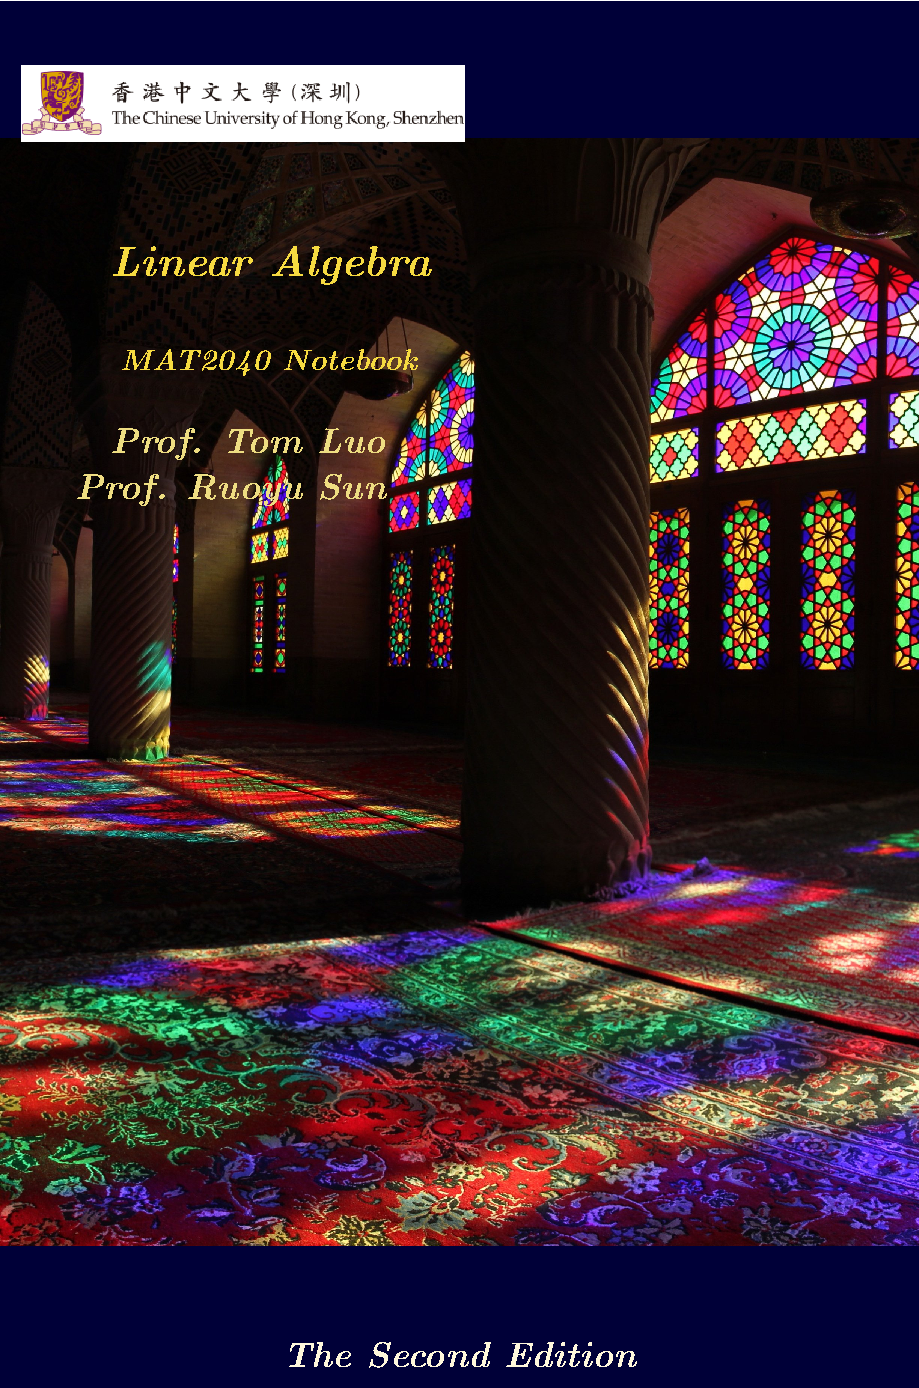
\includepdf[pages={1}]{book_cover/cover/FrontCover}
%%%%%%%%%%%%%%%%%%%%%%%%%%%%%%%%%%%%%%%%%%%%%%%%%%%%%%%%
%% Setting up title pages, type in the appropriate names here:

\booktitle{A Journey \\ In \\
Pure Mathematics}

\subtitle{MAT3006 $\&$ 3040 $\&$ 4002  Notebook}

\AuAff{Dr. Daniel Wong\\ The Chinese University of Hongkong, Shenzhen}
%\AuAff{Prof. Ruoyu Sun\\ University of Illinois Urbana-Champaign}
%% \\ will start a new line.


%% Print Half Title and Title Page:
\halftitlepage
\titlepage

%%%%%%%%%%%%%%%%%%%%%%%%%%%%%%%%%%%%%%%%%%%%%%%%%%%%%%%%
%% Copyright Page
%\begin{copyrightpage}{year}
%Title, etc
%\end{copyrightpage}

% Note, you must use \ to start indented lines, ie,
% 
% \begin{copyrightpage}{2004}
% Survey Methodology / Robert M. Groves . . . [et al.].
% \       p. cm.---(Wiley series in survey methodology)
% \    ``Wiley-Interscience."
% \    Includes bibliographical references and index.
% \    ISBN 0-471-48348-6 (pbk.)
% \    1. Surveys---Methodology.  2. Social 
% \  sciences---Research---Statistical methods.  I. Groves, Robert M.  II. %
% Series.\\
%
% HA31.2.S873 2004
% 001.4'33---dc22                                             2004044064
% \end{copyrightpage}

%%%%%%%%%%%%%%%%%%%%%%%%%%%%%%%%%%%%%%%%%%%%%%%%%%%%%%%%
%% Only Dedication (optional) 
%\dedication{To my girlfriend Jianyu Yang}

\tableofcontents

%\listoffigures %optional
%\listoftables  %optional



% If your book has chapters written by different authors,
% you'll need a Contributors page.

% Use \begin{contributors}...\end{contributors} and
% then enter each author with the \name{} command, followed
% by the affiliation information.

% \begin{contributors}
% \name{Zhi-quan Luo,} Shenzhen Research Institute of Big Data, Lecturer
%
% \name{Ruoyu Sun,} Industrial and Enterprise Systems Engineering, Lecturer
%
% \name{Jie Wang,} The Chinese University of Hongkong, Shenzhen, Typer
% \end{contributors}

%%%%%%%%%%%%%%%%%%%%%%%%%%%%%%%%%%%%%%%%%%%%%%%%%%%%%%%%
% Optional Preface:
%\begin{preface}
%This book is intended for the foundation course MAT2040, which is the first course on the linear algebra. It aims to cover basic linear algebra knowledge and its simple applications. This book was first written in 2017, and it is reviewed and revised in 2018. We have corrected several mistakes shown in the previous book and modified some proofs a little bit to give readers better insights of linear algebra.  During the modification, we also refer to many reading materials, which are also recommended for you:
\begin{itemize}
\item
ENGG 5781 Course Notes by Prof. Wing-Kin (Ken) Ma,  CUHK, Hongkong, China,  http://www.ee.cuhk.edu.hk/$\sim$wkma/engg5781
\item
Roger A. Horn and Charles R. Johnson, Matrix Analysis (Second Edition), Cambridge University Press, 2012.
\item
S. Boyd and L. Vandenberghe, Introduction to Applied Linear Algebra (Vectors, Matrices, and Least Squares), Cambridge University Press, 2018.
\end{itemize}
The whole book can cover a semester course in a 14week, each section in which corresponds to a 2-hour lecture. If you read the whole book, and work some mini-exercises, you will learn a lot. We hope you will get the insights on linear algebra and apply them in your own subject.




%\prefaceauthor{}
%\where{CUHK(SZ)\\
% \today}
%\end{preface}
% ie,
% \begin{preface}
% This is an example preface.
% \prefaceauthor{R. K. Watts}
% \where{Durham, North Carolina\\
% September, 2004}

%%%%%%%%%%%%%%%%%%%%%%%%%%%%%%%%%%%%%%%%%%%%%%%%%%%%%%%%
% Optional Acknowledgments:

\acknowledgments
This book is from the MAT3006,MAT3040,MAT4002 in spring semester, 2018-2019.
\authorinitials{CUHK(SZ)}  


%%%%%%%%%%%%%%%%%%%%%%%%%%%%%%%%%%%%%%%%%%%%%%%%%%%%%%%%
% Optional notations:
\begin{notations}
\acro{$\mathbb{R}^n$}{$n$-dimensional real space}
\acro{$\mathbb{C}^n$}{$n$-dimensional complex space}
\acro{$\mathbb{R}^{m\times n}$}{set of all $m\times n$ real-valued matrices}
\acro{$\mathbb{C}^{m\times n}$}{set of all $m\times n$ complex-valued matrices}
\acro{$x_i$}{$i$th entry of column vector $\bm x$}
\acro{$a_{ij}$}{$(i,j)$th entry of matrix $\bm A$}
\acro{$\bm a_i$}{$i$th column of matrix $\bm A$}
\acro{$\bm a_i\trans$}{$i$th row of matrix $\bm A$}
\acro{$\mathbb{S}^n$}{set of all $n\times n$ real symmetric matrices, i.e., $\bm A\in\mathbb{R}^{n\times n}$ and $a_{ij}=a_{ji}$ for all $i,j$}
\acro{$\mathbb{H}^n$}{set of all $n\times n$ complex Hermitian matrices, i.e., $\bm A\in\mathbb{C}^{n\times n}$ and $\bar{a}_{ij}=a_{ji}$ for all $i,j$}
\acro{$\bm A\trans$}{transpose of $\bm A$, i.e, $\bm B=\bm A\trans$ means $b_{ji}=a_{ij}$ for all $i,j$}
\acro{$\bm A\Her$}{Hermitian transpose of $\bm A$, i.e, $\bm B=\bm A\Her$ means $b_{ji}=\bar{a}_{ij}$ for all $i,j$}
\acro{$\trace(\bm A)$}{sum of diagonal entries of square matrix $\bm A$}
\acro{$\bm 1$}{A vector with all $1$ entries}
\acro{$\bm 0$}{either a vector of all
zeros, or a matrix of all zeros}
\acro{$\bm e_i$}{a unit vector with the nonzero element at the $i$th entry}
\acro{$\mathcal{C}(\bm A)$}{the column space of $\bm A$}
\acro{$\mathcal{R}(\bm A)$}{the row space of $\bm A$}
\acro{$\mathcal{N}(\bm A)$}{the null space of $\bm A$}
\acro{$\Proj_{\mathcal{M}}(\bm A)$}{the projection of $\bm A$ onto the set $\mathcal{M}$}
\end{notations}
\mainmatter
\setcounter{page}{1}

%%%%%%%%%%%%%%%%%%%%%%%%%%%%%%%%%%%%%%%%%%%%%%%%%%%%%%%%
% Optional introduction:
%\begin{introduction}
%
%The word \textit {traffic} becomes \textit {teletraffic} in telecommunications, as communications becomes telecommunications to indicate technology use, e.g., conversation from some distance through phones or Internet. The term teletraffic covers all kinds of computer communication traffic and telecom traffic.  This book includes teletraffic loss models.
%\end{introduction}
\chapter{Week7}
\section{Monday for MAT3040}\index{Monday_lecture}
\paragraph{Reviewing}
Define the characteristic polynomial for an linear operator $T$:
\[
\mathcal{X}_T(x)= \det((T)_{\mathcal{A},\mathcal{A}} - x\bm I)
\]
We will use the notation ``$I/\bm I$'' in two different occasions:
\begin{enumerate}
\item
$I$ denotes the identity transformation from $V$ to $V$ with $I(\bm v)=\bm v,\forall\bm v\in V$
\item
$\bm I$ denotes the identity matrix $(I)_{\mathcal{A},\mathcal{A}}$, defined based on any basis $\mathcal{A}$.
\end{enumerate}

\subsection{Minimal Polynomial}
\begin{definition}[Linear Operator Induced From Polynomial]
Let $f(x):=a_mx^m+\cdots+a_0$ be a polynomial in $\mathbb{F}[x]$, and $T:V\to V$ be a linear operator.
Then the mapping
\[
f(T)=a_mT^m+\cdots+a_1T+a_0I:\quad
V\to V,
\]
is called a linear operator induced from the polynomial $f(x)$.
\end{definition}

\begin{definition}[Minimal Polynomial]
Let $T:V\to V$ be a linear operator.
The \emph{minimal polynomial} $m_T(x)$ is a \emph{nonzero monic polynomial} 
of least (minimal) degree such that 
\[
m_T(T)=\bm0_{V\to V}.
\]
where $\bm0_{V\to V}$ denotes the zero vector in $\text{Hom}(V,V)$.
\end{definition}

\begin{example}
\begin{enumerate}
\item
Let $\bm A=\begin{pmatrix}
1&0\\0&1
\end{pmatrix}$, then $\bm A$ defines a linear operator:
\[
\begin{array}{ll}
A:&\mathbb{F}^2\to\mathbb{F}^2\\
\text{with}&\bm x\mapsto\bm A\bm x
\end{array}
\]
Here $\mathcal{X}_{ A}(x) = (x-1)^2$ and $\bm A-\bm I=\bm0$, which gives $m_A(x)=x-1$.
\item
Let $\bm B=\begin{pmatrix}
1&1\\0&1
\end{pmatrix}$, which implies
\[
\mathcal{X}_{ B}(x)=(x-1)^2,
\]
The question is that can we get the minimal polynomial with degree 1?

The answer is no, since $\bm B-k\bm I=\begin{pmatrix}
1-k&1\\0&1-k
\end{pmatrix}\ne\bm0$.

In fact, $m_B(x) = (x-1)^2$, since
\[
(\bm B-\bm I)^2=\begin{pmatrix}
0&1\\0&0
\end{pmatrix}^2=\begin{pmatrix}
0&0\\0&0
\end{pmatrix}.
\]
\end{enumerate}
\end{example}
%
%\begin{proposition}
%If $\bm A$ and $\bm B$ are similar, then
%\[
%m_{\bm A}(x)=m_{\bm B}(x).
%\]
%\end{proposition}
%\begin{proof}
%Left as exercise.
%\end{proof}
Two questions naturally arises:
\begin{enumerate}
\item
Does $m_T(x)$ exist? If exists, is it unique?
\item
What's the relationship between  $m_T(x)$ and $\mathcal{X}_T(x)$?
\end{enumerate}
Regarding to the first question, the minimal polynomial $m_T(x)$ may not exist, if $V$ has infinite dimension:
\begin{example}
Consider $V=\mathbb{R}[x]$ and the mapping
\[
\begin{array}{ll}
T:&V\to V\\
&p(x)\mapsto\int_0^xp(t)\diff t
\end{array}
\]
In particular, $T(x^n)=\frac{1}{n+1}x^{n+1}$.
Suppose $m_T(x)$ is with degree $n$, i.e., 
\[
m_T(x) = x^n +\cdots+a_1x+a_0,
\]
then 
\[
m_T(T)=T^n+\cdots+a_0I\ \text{is a zero linear transformation}
\]
It follows that
\[
[m_T(T)](x) = \frac{1}{n!}x^n+a_{n-1}\frac{1}{(n-1)!}x^{n-1}+\cdots+a_1x+a_0=0_{\mathbb{F}},
\]
which is a contradiction since
the coefficients of $x^k$ is nonzero on LHS for $k=1,\dots,n$, but zero on the RHS.
\end{example}

\begin{proposition}\label{pro:7:1}
The minimal polynomial $m_T(x)$ always exists for $\dim(V)=n<\infty$.
\end{proposition}
\begin{proof}
It's clear that $\{I,T,\dots,T^n,T^{n+1},\cdots,T^{n^2}\}\subseteq\text{Hom}(V,V).$
Since $\dim(\text{Hom}(V,V))=n^2$, we imply $\{I,T,\dots,T^n,T^{n+1},\cdots,T^{n^2}\}$ is linearly dependent, i.e., there exists $a_i$'s that are not all zero such that
\[
a_0I+a_1T+\cdots+a_{n^2}T^{n^2}=0
\]
i.e., there is a polynomial $g(x)$ of degree less than $n^2$ such that $g(T)=0$.

The proof is complete.
\end{proof}
%\paragraph{Assumption}
%We will asssume $V$ has finite dimension from now on.

\begin{proposition}\label{pro:7:2}
The minimal polynomial $m_T(x)$, if exists, then it exists uniquely.
\end{proposition}
\begin{proof}
Suppose $f_1,f_2$ are two distinct minimal polynomials with $\text{deg}(f_1)=\text{deg}(f_2)$.
It follows that
\begin{itemize}
\item
$\text{deg}(f_1-f_2)<\text{deg}(f_1)$.
\item
$f_1-f_2\ne0$
\item
$(f_1-f_2)(T) = f_1(T) - f_2(T)=0_{V\to V}$
\end{itemize}
By scaling $f_1-f_2$, there is a monic polynomial $g$ with lower degree satisfying $g(T)=0,$
which contradicts the definition for minimal polynomial.
\end{proof}

\begin{proposition}\label{pro:7:3}
Suppose $f(x)\in\mathbb{F}[x]$ satisfying $f(T)=\bm0$, then
\[
m_T(x)\mid f(x).
\]
\end{proposition}
\begin{proof}
It's clear that $\text{deg}(f)\ge\text{deg}(m_T)$.
The division algorithm gives 
\[
f(x)=q(x)m_T(x)+r(x).
\]
Therefore, for any $\bm v\in V$
\[
[r(T)](\bm v) = [f(T)](\bm v) - [q(T)m_T(T)](\bm v)=\bm0_V-q(T)\bm0_{V}=\bm0_V-\bm0_V=\bm0_{V}
\]
Therefore, $r(T) = \bm0_{V\to V}$.
By definition of minimal polynomial, we imply $r(x)\equiv0$.
\end{proof}
\begin{proposition}\label{pro:7:4}
If $\bm A,\bm B\in\mathbb{F}^{n\times n}$ are similar to each other, then $m_A(x) = m_B(x)$.
\end{proposition}
\begin{proof}
Suppose that $\bm B= \bm P^{-1}\bm A\bm P$, and that 
\[
\begin{array}{ll}
m_A(x)=x^k+\cdots+a_1x+a_0,
&
m_B(x)=x^{\ell}+\cdots+b_0.
\end{array}
\]
It follows that
\begin{align*}
m_A(\bm B)&=\bm B^k+\cdots+a_0I\\
&=\bm P^{-1}\bm A^k\bm P+\cdots+a_0\bm P^{-1}\bm P\\
&=\bm P^{-1}(\bm A^k+\cdots+a_0\bm I)\bm P\\
&=\bm P^{-1}(m_{A}(\bm A))\bm P
\end{align*}
Therefore, $m_A(\bm B)=\bm0$ since $m_{A}(\bm A)=\bm0$. By proposition~(\ref{pro:7:3}), we imply $m_{B}(x)\mid m_{A}(x)$. 
Similarly, $m_A(x)\mid m_B(x)$. 
Since $m_A(x)$ and $m_B(x)$ are monic, we imply $m_A(x)=m_B(x)$.
\end{proof}
\begin{remark}
Proposition~(\ref{pro:7:4}) claims that the minimal polynomial is \emph{similarity-invariant}; actually, the characteristic polynomial is \emph{similarity-invariant} as well.
\end{remark}
\paragraph{Assumption}
We will asssume $V$ has finite dimension from now on.
Now we study the vanishing of a single vector $\bm v\in V$.
\paragraph{Notation}
The $m_T(x)$ is a nonzero monic poylnomial of least degree such that 
\[
m_T(T)=\bm0_{V\to V}.
\]
\subsection{Minimal Polynomial of a vector}

\begin{definition}[Minimal Polynomial of a vector]
Similar to the minimal polynomial, we define the \emph{minimal polynomial of a vector $\bm v$ relative to $T$}, say $m_{T,\bm v}(x)$, as the monic polynomial of least degree such that 
\[
m_{T,\bm v}(T)(\bm v)=0
\]
\end{definition}
The existence of minimal polynomial of a vector is due to the existence of minimal polynomial; the uniqueness follows similarly as in proposition~(\ref{pro:7:2}).

\begin{proposition}
Let $T:V\to V$ be a linear operator and $\bm v\in V$.
The degree of the minimal polynomial of a vector is upper bounded by:
\[
\text{deg}(m_{T,\bm v}(x))\le \dim (V).
\]
\end{proposition}
\begin{proof}
It's clear that $\{\bm v,T\bm v,\dots,T^n\bm v\}\subseteq V$ and the proof follows similarly as in proposition~(\ref{pro:7:1}).
\end{proof}

Similar to the division property in proposition~(\ref{pro:7:3}), we have the division proprty for minimal polynomial of a vector:
\begin{proposition}\label{pro:7:6}
Suppose $f(x)\in\mathbb{F}[x]$ satisfying $f(T)(\bm v)=\bm0_{V}$, then
\[
m_{T,\bm v}(x)\mid f(x).
\]
In particular, $m_{T,\bm v}\mid m_T(x)$.
\end{proposition}

\begin{proof}
The proof follows similarly as in proposition~(\ref{pro:7:3}).
\end{proof}

\begin{proposition}
Suppose that $m_{T,\bm v}(x)= f_1(x)f_2(x)$, where $f_1,f_2$ are both monic. Let $\bm w = f_1(T)\bm v$, then
\[
m_{T,\bm w}(x) = f_2(x)
\]
\end{proposition}
\begin{proof}
\begin{enumerate}
\item
\[
f_2(T)\bm w = f_2(T)f_1(T)\bm v = m_{T,\bm v}(T)\bm v=\bm0
\]
By the proposition~(\ref{pro:7:3}), we imply 
$
m_{T,\bm w}|f_2
$.
\item
On the other hand,
\[
\bm0 = m_{T,\bm w}(T)(\bm w) = m_{T,\bm w}(T)f_1(T)\bm v= f_1(T)m_{T,\bm w}(T)\bm v,
\]
which implies that $m_{T,\bm v}(x)\mid f_1(x)m_{T,\bm w}(x),$, i.e.,
\[
f_1\cdot f_2\mid f_1\cdot m_{T,\bm w}\implies
f_2\mid m_{T,\bm w}.
\]
The proof is complete.
\end{enumerate}
\end{proof}
















\section{Monday for MAT3006}\index{Monday_lecture}
\paragraph{Reviewing}
\begin{enumerate}
\item
Compactness/Sequential Compactness:
\begin{itemize}
\item
Equivalence for metric space
\item
Stronger than closed and bounded
\end{itemize}
\item
Completeness: 
\begin{itemize}
\item
The metric space $(E,d)$ is complete if every Cauchy sequence on $E$ is convergent.
\item
$\mathbb{P}[a,b]\subseteq\mathcal{C}[a,b]$ is not complete:
\[
f_N(x)=\sum_{n=0}^N(-1)^n\frac{x^{2n}}{(2n)!}\to\cos x,
\]
while $\cos x\notin\mathcal{P}[a,b]$.
\end{itemize}
\end{enumerate}


\subsection{Remarks on Completeness}

\begin{proposition}
Let $(X,d)$ be a metric space.
\begin{enumerate}
\item
If $X$ is complete and $E\subseteq X$ is closed, then $E$ is complete.
\item
If $E\subseteq X$ is complete, then $E$ is closed in $X$.
\item
If $E\subseteq X$ is compact, then $E$ is complete.
\end{enumerate}
\end{proposition}
\begin{proof}
\begin{enumerate}
\item
Every Cauchy sequence $\{e_n\}$ in $E\subseteq X$ is also a Cauchy sequence in $E$.

Therefore we imply $\{e_n\}\to x\in X$, due to the completeness of $X$.

Due to the closedness of $E$, the limit $x\in E$, i.e., $E$ is complete.
\item
Consider any convergent sequence $\{e_n\}$ in $E$, with some limit $x\in X$.

We imply $\{e_n\}$ is Cauchy and thus $\{e_n\}\to e\in E$, due to the completeness of $E$.

By the uniqueness of limits, we must have $x=z\in E$, i.e., $E$ is closed.
\item
Consider a Cauchy sequence $\{e_n\}$ in $E$.
There exists a subsequence $\{e_{n_j}\}\to e\in E$, 
due to the sequential compactness of $E$.

It follows that for large $n$ and $j$,
\[
d(e_n,e)
\makebox[1cm][c]{$\overset{\text{(a)}} \leq$}
 d(e_n,e_{n_j})+d(e_{n_j},e)
 \makebox[1cm][c]{$\overset{\text{(b)}} <$}
 \varepsilon
\]
where (a) is due to triangle inequality
and (b) is due to the Cauchy property of $\{e_n\}$ and the convergence of $\{e_{n_j}\}$. 

Therefore, we imply $\{e_n\}\to e\in E$, i.e., $E$ is complete.
\end{enumerate}
\end{proof}

\begin{remark}
Given any metric space that may not be necessarily complete, we can make the union of it with another space to make it complete, e.g., just like the completion from $\mathbb{Q}$ to $\mathbb{R}$.
\end{remark}


\subsection{Contraction Mapping Theorem}

The motivation of the contraction mapping theorem comes from solving an equation $f(x)$. More precisely, such a problem can be turned into a problem for fixed points, i.e., it suffices to find the fixed points for $g(x)$, with $g(x)=f(x)+x$.

\begin{definition}
Let $(X,d)$ be a metric space. 
A map $T:(X,d)\to (X,d)$ is a \emph{contraction} 
if there exists a constant $\tau\in(0,1)$ such that
\[
\begin{array}{ll}
d(T(x),T(y))<\tau\cdot d(x,y),
&
\forall x,y\in X
\end{array}
\]
A point $x$ is called a fixed point of $T$ if $T(x)=x$.
\end{definition}
\begin{remark}
All contractions are continuous: 
Given any convergence sequence $\{x_n\}\to x$, 
for $\varepsilon>0$, take $N$ such that 
$d(x_n,x)<\frac{\varepsilon}{\tau}$ for $n\ge N$. It suffices to show the convergence of $\{T(x_n)\}$:
\[
d(T(x_n),T(x))<\tau\cdot T(x_n,x)<\tau\cdot\frac{\varepsilon}{\tau}=\varepsilon.
\]
Therefore, the contraction is Lipschitz continuous with Lipschitz constant $\tau$.
\end{remark}

\begin{theorem}[Contraction Mapping Theorem / Banach Fixed Point Theorem]
Every contraction $T$ in a \emph{complete} metric space $X$ has a unique fixed point.
\end{theorem}

\begin{example}
\begin{enumerate}
\item
The mapping $f(x)=x+1$ is not a contraction in $X=\mathbb{R}$, and it has no fixed point.
\item
Consider an in-complete space $X=(0,1)$ and a contraction $f(x)=\frac{x+1}{2}$. It doesn't admit a fixed point on $X$ as well.
\end{enumerate}
\end{example}

\begin{proof}
Pick any $x_0\in X$, and define a sequence recursively by setting $x_{n+1}=T(x_n)$ for $n\ge0$.
\begin{enumerate}
\item
Firstly show that the sequence $\{x_n\}$ is Cauchy.

We can upper bound the term $d(T^n(x_0),T^{n-1}(x_0))$:
\begin{equation}\label{Eq:3:4}
d(T^n(x_0),T^{n-1}(x_0))\le \tau d(T^{n-1}(x_0),T^{n-2}(x_0))\le\cdots\le \tau^{n-1}d(T(x_0),x_0)
\end{equation}
Therefore for any $n\ge m$, where $m$ is going to be specified later,
\begin{subequations}
\begin{align}
d(x_n,x_m)&=d(T^n(x_0),T^m(x_0))\label{Eq:3:5:a}\\
&\le\tau d(T^{n-1}(x_0),T^{m-1}(x_0))\le\cdots\le\tau^md(T^{n-m}(x_0),x_0)\label{Eq:3:5:b}\\
&\le\tau^m\sum_{j=1}^{n-m}\tau^{n-m-j}d(T(x_0),x_0)\label{Eq:3:5:c}\\
&<\frac{\tau^{m}}{1-\tau}d(T(x_0),x_0)\label{Eq:3:5:d}\\
&\le\varepsilon\label{Eq:3:5:e}
\end{align}
\end{subequations}
where (\ref{Eq:3:5:b}) is by repeatedly applying contraction property of $d$; (\ref{Eq:3:5:c}) is by applying the triangle inequality and (\ref{Eq:3:4}); (\ref{Eq:3:5:e}) is by choosing sufficiently large $m$ such that $\frac{\tau^{m}}{1-\tau}d(T(x_0),x_0)<\varepsilon$.

Therefore, $\{x_n\}$ is Cauchy. By the completeness of $X$, we imply $\{x_n\}\to x\in X$.
\item
Therefore, we imply 
\[
x=\lim_{n\to\infty}x_{n+1}=\lim_{n\to\infty}T(x_n)=T(\lim_{n\to\infty}x_n)=T(x),
\]
i.e., $x$ is a fixed point of $T$.

Now we show the uniqueness of the fixed point. Suppose that there is another fixed point $y\in X$, then
\[
d(x,y)=d(T(x),T(y))<\tau\cdot d(x,y)\implies d(x,y)<\tau d(x,y),\quad\tau\in(0,1),
\]
and we conclude that $d(x,y)=0$, i.e., $x=y$.
\end{enumerate}
\end{proof}

\begin{example}[Convergence of Newton's Method]
The Newton's method aims to find the root of $f(x)$ by applying the iteration
\[
x_{n+1}=x_n-\frac{f(x_n)}{f'(x)}
\]
Suppose $r$ is a root for $f$, the pre-assumption for the convergence of Newton's method is:
\begin{enumerate}
\item
$f'(r)\ne0$
\item
$f\in\mathcal{C}^2$ on some neighborhood of $r$
\end{enumerate}
\begin{proof}
\begin{enumerate}
\item
We first show that there exists $[r-\varepsilon,r+\varepsilon]$ such that the mapping
\[
\begin{array}{ll}
T:\mathcal{C}[r-\varepsilon,r+\varepsilon]\to\mathbb{R},
&
f(x)\mapsto x-\frac{f(x)}{f'(x)}
\end{array}
\]
satisfies $|T'(x)|<1$ for $\forall x\in[r-\varepsilon,r+\varepsilon]$:

Note that $T'(x)=\frac{f(x)}{[f'(x)]^2}f''(x)$, and we define $h(x)=|T'(x)|$.

It's clear that $h(r)=0$ and $h(x)$ is continuous, which implies
\[
r\in h^{-1}((-1,1))\implies
B_\rho(r)\subseteq h^{-1}((-1,1))\ \text{for some $\rho>0$}.
\]
Or equivalently, $h((r-\rho,r+\rho))\subseteq(-1,1)$. Take $\varepsilon=\frac{\rho}{2}$, and the result is obvious.
\item
Therefore, any $x,y\in [r-\varepsilon,r+\varepsilon]$,
\begin{subequations}
\begin{align}
d(T(x),T(y)):&=|T(x)-T(y)|\label{Eq:3:6:a}\\
&=|T'(\xi)||x-y|\label{Eq:3:6:b}\\
&\le\max_{\xi\in [r-\varepsilon,r+\varepsilon]}|T'(\xi)||x-y|\label{Eq:3:6:c}\\
&<m\cdot|x-y|\label{Eq:3:6:d}
\end{align}
\end{subequations}
where (\ref{Eq:3:6:b}) is by applying MVT, and $\xi$ is some point in $[r-\varepsilon,r+\varepsilon]$; we assume that $\max_{\xi\in [r-\varepsilon,r+\varepsilon]}|T'(\xi)|<m$ for some $m<1$ in (\ref{Eq:3:6:d}).
\end{enumerate}
Therefore, $T\in\mathcal{C}[r-\varepsilon,r+\varepsilon]$ is a contraction. By applying the contraction mapping theorem, there exists a unique fixed point near $[r-\varepsilon,r+\varepsilon]$:
\[
x-\frac{f(x)}{f'(x)}=x\implies\frac{f(x)}{f'(x)}=0\implies f(x)=0,
\]
i.e., we obtain a root $x=r$.
\end{proof}

Summary: if we use Newton's method on any point between $[r-\varepsilon,r+\varepsilon]$ where $f(r)=0$ and $\varepsilon$ is sufficiently small, then we will eventually get close to $r$.
\end{example}

\subsection{Picard Lindelof Theorem}
We will use Banach fixed point theorem to show the existence and uniqueness of the solution of ODE
\begin{equation}\label{Eq:3:7}
\left\{
\begin{aligned}
\frac{\diff y}{\diff x}&=f(x,y(x))\\
y(x_0)&=y_0
\end{aligned}
\right.\qquad
\textbf{Initial Value Problem, IVP}
\end{equation}
\begin{example}
Consider the IVP
\[
\left\{
\begin{aligned}
\frac{\diff y}{\diff x}&=x^{2}y^{1/5}\\
y(x_0)&=c>0
\end{aligned}
\right.
\implies 
y=\left(
\frac{4x^3}{15}+c^{4/5}
\right)^{5/4}
\]
which can be solved by the separation of variables:
\[
c>0\implies y=\left(
\frac{4x^3}{15}+c^{4/5}
\right)^{5/4}.
\]
However, when $c=0$, the ODE does not have a unique solution. One can verify that $y_1,y_2$ given below are both solutions of this ODE:
\[
y_1=(\frac{4x^3}{15})^{5/4},\qquad
y_2=0
\]
This example shows that even when $f$ is very nice, the IVP may not have unique solution. The Picard-Lindelof theorem will give a clean condition on $f$ ensuring the unique solvability of the IVP~(\ref{Eq:3:7}).
\end{example}



\section{Monday for MAT4002}\index{Monday_lecture}
There will be a quiz next Monday. The scope is everything before CNY holiday. There will be one question with four parts for 40 minutes.
\subsection{Hausdorffness}
\paragraph{Reviewing}
A topological space $(X,\mathcal{T})$ is said to be \emph{Hausdorff} (or satisfy the second separtion property), if given any distinct points $x,y\in X$, there exist disjoint open sets $U,V$ such that $U\ni x$ and $V\ni y$.

\begin{proposition}
If the topological space $(X,\mathcal{T})$ is Hausdorff,
then all sequences $\{x_n\}$ in $X$ has at most one limit.
\end{proposition}
\begin{proof}
Suppose on the contrary that 
\[
\{x_n\}\to a,\quad
\{x_n\}\to b,\text{ with }a\ne b
\]
By separation property, there exists 
$U,V\in\mathcal{T}$ and $U\cap V=\emptyset$ 
such that $U\ni a$ and $V\ni b$.

By tje openness of $U$, there exists $N$ such that $\{x_N,x_{N+1},\dots\}\subseteq U$, since $\{x_n\}\to a\in U$. Similarly, there exists $M$ such that $\{x_M,x_{M+1},\dots\}\subseteq V$. Take $K=\max\{M,N\}+1$, then $\emptyset\ne U\cap V\ni x_K$, which is a contradiction.
\end{proof}

\begin{proposition}
Let $X,Y$ be Hausdorff spaces. Then $X\times Y$ is Hausdorff with product topology.
\end{proposition}
\begin{proof}
Suppose that $(x_1,y_1)\ne (x_2,y_2)$ in $X\times Y$.
Then $x_1\ne x_2$ or $y_1\ne y_2$.
w.l.o.g., assume that $x_1\ne x_2$, then there exists $U,V$ open in $X$ such that
$x_1\in U, x_2\in V$ with $U\cap V=\emptyset$.

Therefore, we imply $(U\times Y), (V\times Y)\in\mathcal{T}_{X\times Y}$, and
\[
(U\times Y)\cap(V\times Y) = (U\cap V)\cap Y=\emptyset
\]
with $(x_1,y_1)\in U\times Y, (x_2,y_2)\in V\times Y$, i.e., $X\times Y$ is Hausdorff with product topology.
\end{proof}
The same argument applies if the second separation property is replaced by first separation property.

\begin{proposition}
If $f:X\to Y$ is an injective continuous mapping, then $Y$ is Hausdorff implies $X$ is Hausdorff.
\end{proposition}
\begin{proof}
Suppose that $Y$ satisfies the second separation property. For given $a\ne b$ in $X$, we imply $f(a)\ne f(b)$ in $Y$. Therefore, there exists $U\ni f(a),V\ni f(b)$ with $U\cap V=\emptyset$. It follows that
\[
\begin{array}{ll}
a\in f^{-1}(U),b\in f^{-1}(V),
&
f^{-1}(U)\cap f^{-1}(V) = f^{-1}(U\cap V)=\emptyset,
\end{array}
\]
i.e., $X$ is Hausdorff.
\end{proof}

\begin{corollary}
If $f:X\to Y$ is homeomorphic, then $X$ is Hausdorff iff $Y$ is Hausdorff, i.e., 
Hausdorffness is a topological property 
(i.e., a property that is preserved under homeomorphism).
\end{corollary}

\subsection{Connectedness}
\begin{definition}[Connected]
The topological space $(X,\mathcal{T})$ is \emph{disconnected} if there are open $U,V\in\mathcal{T}$ such that
\begin{equation}\label{Eq:3:13}
\begin{array}{lll}
U\ne\emptyset,
V\ne\emptyset,
&
U\cap V=\emptyset,
&
U\cup V = X.
\end{array}
\end{equation}
If no such $U,V\in\mathcal{T}$ exist, then $X$ is \emph{connected}.
\end{definition}

\begin{proposition}
Let $(X,\mathcal{T})$ be topological spaces.
TFAE (i.e., the followings are equivalent):
\begin{enumerate}
\item
$X$ is connected
\item
The \emph{only} subset of $X$ which are both open and closed are $\emptyset$ and $X$
\item
Any continuous function $f:X\to\{0,1\}$ ($\{0,1\}$ is equipped with discrete topology) is a constant function.
\end{enumerate}
\end{proposition}
\begin{proof}
(1) implies (2): Suppose that $U\subseteq X$ is both open and closed. 
Then $U,X\setminus U$ are both open and disjoint, and $U\cup(X\setminus U) = X$.
By connnectedness, either $U=\emptyset$ or $X\setminus U=\emptyset$.
Therefore, $U=\emptyset$ or $X$.

(2) implies (3): 
Note that  $U = f^{-1}(\{0\})$ and $V = f^{-1}(\{1\})$ are open disjoint sets in $X$ satisfying $U\cup V = X$.
By the connectedness of $X$, either $(U,V)=(X,\emptyset)$ or $(V,U)=(\emptyset,X)$. In either case, we imply $f$ is a constant function.


(3) implies (2): 
Suppose that $U\subseteq X$ is both open and closed. 
Construct the mapping
\[
f(x) = \left\{
\begin{aligned}
0,&\quad x\in U\\
1,&\quad x\in X\setminus U
\end{aligned}
\right.
\]
It's clear that $f$ is continuous, and therefore $f(x)=0$ or $1$. 
Therefore $U=\emptyset$ or $X$.

(2) implies (1): Suppose on the contrary that there exists open $U,V$ such that (\ref{Eq:3:13}) holds. By (\ref{Eq:3:13}), we imply $U=X\setminus V$ is closed as well. Since $U\ne\emptyset$ and $U=\emptyset$ or $X$, we imply $U=X$, which implies $V=\emptyset$, which is a contradiction.
\end{proof}

\begin{corollary}
The interval $[a,b]\subseteq\mathbb{R}$ is connnected
\end{corollary}
\begin{proof}
Suppose on the contrary that there exists continuous function $f:[a,b]\to\{0,1\}$ that takes 2 values. Construct the mapping $\tilde f:[a,b]\to\mathbb{R}$
\[
\begin{array}{ll}
&\tilde f:
[a,b]
\xrightarrow{f}\{0,1\}
\xrightarrow{i}
\mathbb{R},\\
\text{with}&\tilde{f} = i\circ f.
\end{array}
\]
Note that $\{0,1\}\subseteq \mathbb{R}$ denotes the subspace topology, we imply the inclusion mapping $i:\{0,1\}\to \mathbb{R}$ with $s\mapsto s$ is continuous. The composition of continuous mappings is continuous as well, i.e., $\tilde{f}$ is continuous.

Since the function $f$ can take two values, there exists $p,q\in[a,b]$ such that $\tilde{f}(p)=i\circ f(p)=0$ and $\tilde{f}(q)=i\circ f(q)=1$. 
By intermediate value theorem, there exists $r\in[a,b]$ such that 
$\tilde f(r) = i\circ f(r)=1/2$, which implies $f(r)=\frac{1}{2}$, which is a contradiction.
\end{proof}

\begin{definition}[Connected subset]
A non-empty subset $S\subseteq X$ is \emph{connected} if 
$S$ with the subspace topology is connected 

Equivalently, $S\subseteq X$ is connected if,
whenever $U,V$ are open in $X$ such that $S\subseteq U\cup V$, and 
$
(U\cap V)\cap S=\emptyset
$, one can imply either $U\cap S=\emptyset$ or $V\cap S=\emptyset$.
\end{definition}

\begin{proposition}\label{pro:4:9}
If $f:X\to Y$ is continuous mapping, and the subset $A\subseteq X$ is connected, then $f(A)$ is connected. 
In other words, the continuous image of a connected set is connected.
\end{proposition}

\begin{proof}
Suppose that $U,V\subseteq Y$ is open such that
\[
\begin{array}{ll}
f(A)\subseteq U\cup V,
&
(U\cap V)\cap f(A)=\emptyset.
\end{array}
\]
Therefore we imply 
\[
\begin{array}{ll}
A\subseteq f^{-1}(U)\cup f^{-1}(V),
&
(f^{-1}(U)\cap A)\cap(f^{-1}(V)\cap A)=\emptyset
\end{array}
\]
By connectedness of $A$, either $f^{-1}(U)\cap A=\emptyset$ or $f^{-1}(V)\cap A=\emptyset$. 
Therefore, $f(A)\cap U=\emptyset$ or $f(A)\cap V=\emptyset$, i.e., $f(A)$ is connected.
\end{proof}

\begin{proposition}\label{pro:4:10}
If $\{A_i\}_{i\in I}$ are connnected and $A_i\cap A_j\ne\emptyset$ for $\forall i,j\in I$, then the set $\bigcup_{i\in I}A_i$ is connected.
\end{proposition}

\begin{proof}
Suppose the function $f:\cup_{i\in I}A_i\to\{0,1\}$ is a continuous map. Then we imply that its restriction $f|_{A_i} = f\circ i: A_i\to\{0,1\}$ is continuous for all $i\in I$. Thus $f|_{A_i}$ is a constant for all $i\in I$. Due to the non-empty intersection of $A_i,A_j$ for $\forall i,j\in I$, we imply $f$ is constant.
\end{proof}

\begin{proposition}
If $X,Y$ are connnected, then $X\times Y$ is connected using product topology.
\end{proposition}
\begin{proof}
It's clear that $X\times \{y_0\}$ is connected in $X\times Y$ for fixed $y_0$; and $\{x_0\}\times Y$ is connected for fixed $x_0$.

Therefore, for fixed $y_0\in Y$, construct $B=X\times \{y_0\}$ and $C_x=\{x\}\times Y$, which follows that
\[
B\cap C_x=\{(x,y_0)\}\ne\emptyset,\forall x\in X\implies
B\cup\left\{\bigcup_{x\in X}C_x\right\}=X\times Y\text{ is connected.}
\]
\end{proof}

\begin{definition}[Path Connectes]
Let $(X,\mathcal{T})$ be a topological space. 
\begin{enumerate}
\item
A path connecting 2 points $x,y\in X$ is a continuous function $\tau:[0,1]\to X$ with $\tau(0)=x,\tau(1)=y$.
\item
$X$ is path-connected if any 2 points in $X$ can be connected by a path.
\item
The set $A\subseteq X$ is path-connected, if $A$ sastisfies the condition using subspace topology.

Or equivalently,  $A$ is path-connected if for any 2 points in $X$, there exists a continuous $t:[0,1]\to X$ with $t(x)\in A$ for any $x$, connecting the 2 points.
\end{enumerate}
\end{definition}


























\backmatter
%\appendix
\chapter{This is Appendix Title}

\section{This is First Level Heading}
\lipsum[1-2]

\subsection{This is Second Level Heading}
\lipsum[3]

\subsubsection{This is Third Level Heading}
\lipsum[4]

\paragraph{This is Fourth Level Heading}
\lipsum[5]

\subparagraph{This is Fifth Level Heading}
\lipsum[6]
\begin{theorem}
asfasf
\end{theorem}
\begin{theorem}
asfasf
\end{theorem}
%\backmatter

%\bibliography{wiley}%


%
\includegraphics{AuthorIcon}

\latexprintindex

\end{document} 
